%\documentclass[12pt,papel,twoside]{ibtesis}
\documentclass[12pt,screen,twoside,pagebackref]{ibtesis}
% \documentclass[12pt,papel,singlespace,oneside]{ibtesis}
% \documentclass[12pt,papel,preprint,singlespace,oneside]{ibtesis}
\usepackage{ibextra}
\usepackage{listings}
\makeatletter
\renewcommand*{\backref}[1]{}
\renewcommand*{\backrefalt}[4]{}
\makeatother
\renewcommand{\lstlistingname}{Código}
\lstset{
  captionpos=b   % "b" de "bottom"
}
%%%%%%%%%%%%%%%%%%%%%%%%%%%%%%%%%%%%%%%%%%%%%%%%%%%%%%%%%%%%%%%%%%%%%%%%%%%%%%%%
%%%%%%%%%%%%%%%%%%%%% Informacion sobre la tesis %%%%%%%%%%%%%%%%%%%%%%%%%%%%%%%
\title{Patrones de interacción espacio-temporal de animales en su hábitat natural}
\author{Luciano Carlos Lopez Bertazza}
\director{Dra. Karina Laneri, Dr. David Alonso}
\carrera{Tesis Carrera de Licenciatura en F\'{\i}sica}
\grado{Licenciatura en Física}
\laboratorio{Física Estadística e Interdisciplinaria -- Centro At\'{o}mico Bariloche}
\jurado{Dr. Guillermo Abramson (Instituto Balseiro, Centro At\'{o}mico Bariloche) \\ 
Dr.~Luiz Menon Junior (Instituto Balseiro, Centro At\'{o}mico Bariloche)\\
Mg.~Jorge Cogo (Universidad Nacional de Río Negro, Instituto Balseiro, Centro At\'{o}mico Bariloche)\\
}
\palabrasclave{comportamiento animal, movimiento subdifusivo, leyes de potencias, simulaciones estocásticas, \textit{Chelonoidis chilensis}.}
\keywords{animal behavior, subdiffusive movement, power laws, stochastic simulations, \textit{Chelonoidis chilensis}.}
% Si queremos poner la fecha manualmente:
% \date{Diciembre de 2099}

%%%%%%%%%%%%%%%%%%%%%%%%%%%%%%%%%%%%%%%%%%%%%%%%%%%%%%%%%%%%%%%%%%%%%%%%%%%%%%%%
%\titlepagefalse % Si no quiere compilar la portada descomente esta linea
%\includeonly{apendices} % Compilar s\'{o}lo estos archivos 
\graphicspath{{figs/}} % Lugar donde encontrar las figuras generales (se puede poner uno en cada cap{\'{\i}}tulo)
%%%%%%%%%%%%%%%%%%%%%%%%%%%%%%%%%%%%%%%%%%%%%%%%%%%%%%%%%%%%%%%%%%%%%%%%%%%%%%%%


\begin{document}

% Dentro del environment 'preliminary' va:
% la dedicatoria, resumen, abstract, indices

\begin{preliminary}

% Escriba su dedicatoria
\dedicatoria{
A ....\\
}

%%% \'{I}ndices %%%%

\begin{abreviaturas}
\begin{description}
    \item[GPS] Global Positioning System (Sistema de Posicionamiento Global)
\end{description}
\end{abreviaturas}

\tableofcontents                %\'{I}ndice

\listoffigures                  %Figuras

\listoftables                   %Tablas

\begin{resumen}%
\end{resumen}

\begin{abstract}%
\end{abstract}




%%% Local Variables: 
%%% mode: latex
%%% TeX-master: "template"
%%% End: 


\end{preliminary}


% Podemos usar cualquiera de los dos comandos: \input o \include para incluir el texto
\chapter{Introducción y metodología}\label{Introduccion}
\chapterquote{}{}

\section{Motivación}\label{I:mot}
La ciencia no avanza únicamente a través de grandes descubrimientos disruptivos, sino también mediante la acumulación de pequeños aportes que, 
en conjunto, terminan generando un impacto significativo. En esta línea, el estudio del comportamiento animal, y en especial su movimiento, 
no suele ser más que un granito de arena en el conjunto de técnicas y herramientas que los conservacionistas utilizan para proteger a las 
especies, entendiendo cómo interactúan con otros individuos, cómo utilizan su hábitat y cómo se adaptan ante el cambio del mismo. 
En el caso de la tortuga terrestre argentina, \textit{Chelonoidis chilensis}, estos aportes cobran relevancia, dado su estado de vulnerabilidad 
y el escaso conocimiento cuantitativo sobre la misma.

El objetivo generar de esta tesis es estudiar y replicar el comportamiento de estas tortugas en su hábitat natural, con el objetivo de entender mejor su estrategia
de movimiento y su interacción con el entorno que las rodea. Para ello, se dispone de un conjunto de datos obtenidos mediante rastreadores de GPS,
que permiten registrar la posición de los animales a lo largo del tiempo. Adicionalmente, se toma como principal inspiración el trabajo realizado
por C. Callenbach et al. \cite{callenbach2025}, quienes aplicaron técnicas de aprendizaje automático para clasificar los patrones de movimiento de 
tortugas en cautiverio y en su hábitat natural.

\section{Tortuga terrestre argentina: \textit{Chelonoidis chilensis}}\label{I:tortuga}

El objeto de estudio de esta tesis es la tortuga terrestre argentina, \textit{Chelonoidis chilensis}, una especie clasificada como ``En Peligro''
en la lista roja de la \textit{International Union for Conservation of Nature} (IUCN) \cite{kubisch2023chelonoidis}. Esta clasificación se ve impulsada especialmente 
por la expansión ganadera, que se encarga de segmentar y deteriorar su hábitat, y por la captura y venta ilegal de los individuos. En adición, la 
introducción de nuevos depredadores como el jabalí (\textit{Sus scrofa}) \cite{kubisch2014} pone en tensión la ya de por sí delicada población de tortugas. 
Estos reptiles son nativos de Sudamérica, abarcando gran parte de Argentina, el sur de Bolivia y el norte de Paraguay, como se observa en la Figura \ref{fig:mapa}. 

\begin{figure}[ht]
    \centering
    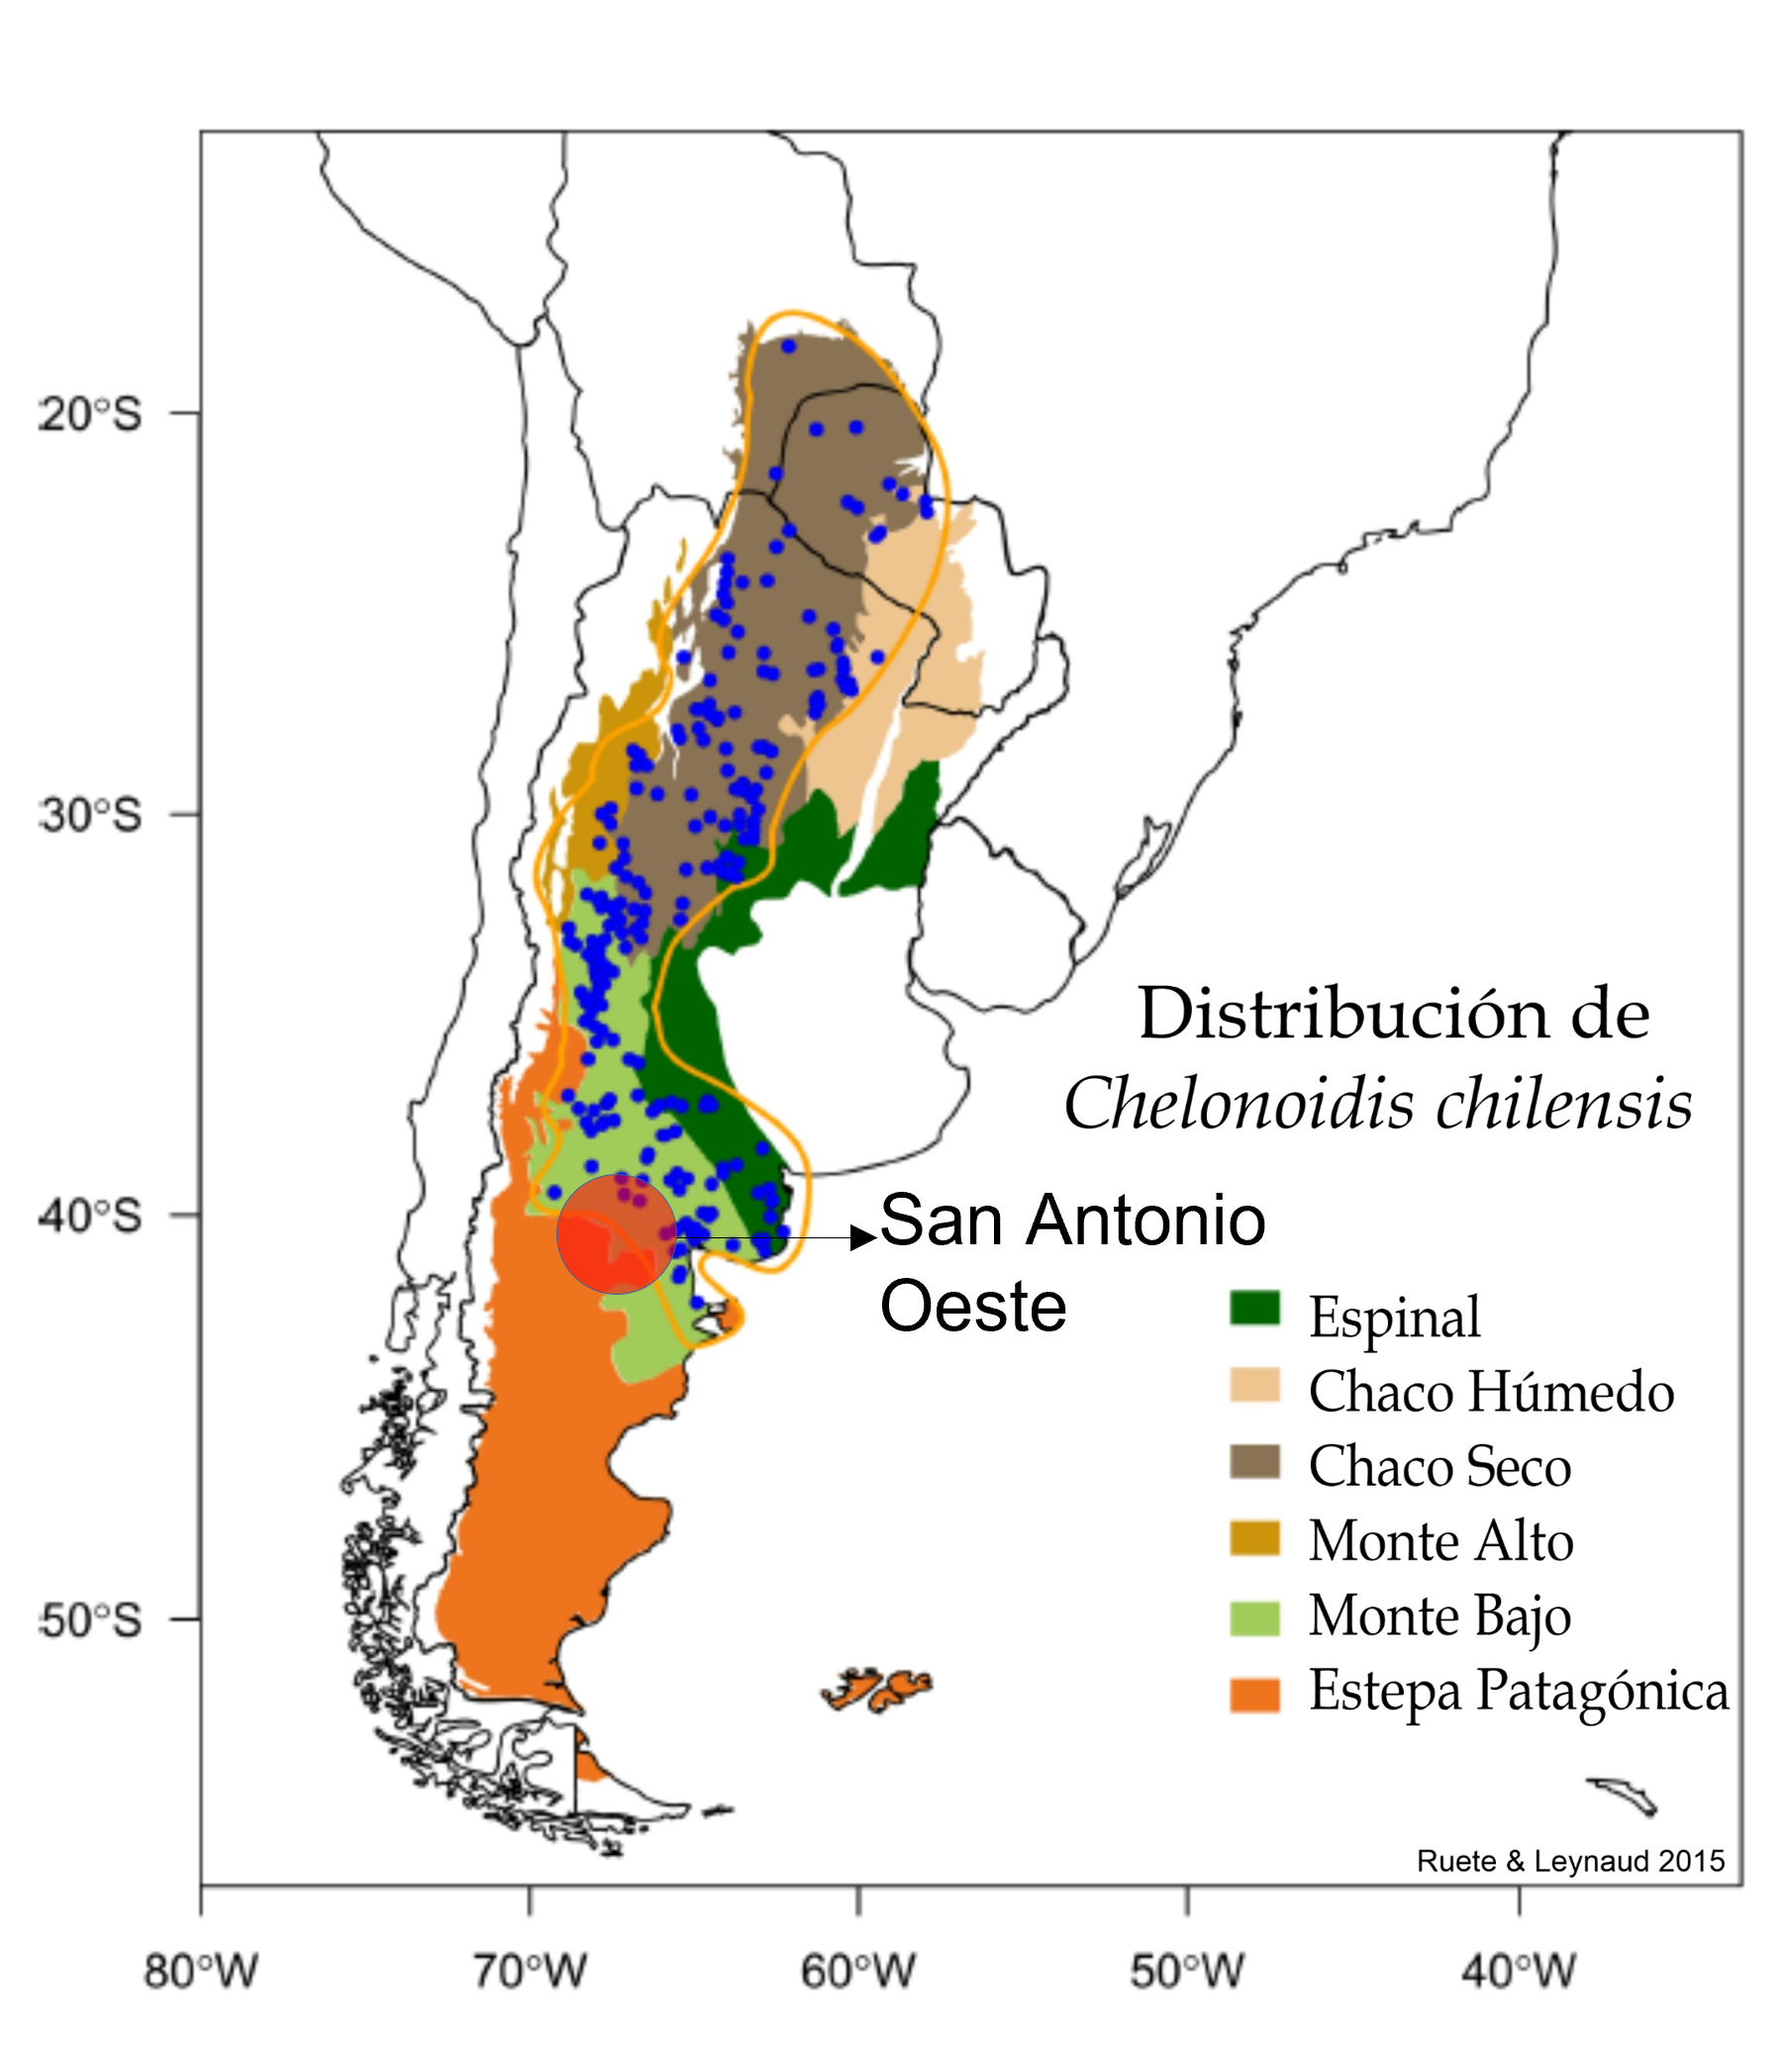
\includegraphics[scale=0.8]{figs/mapa.png}
    \caption{Distribución geográfica de la tortuga terrestre argentina, \textit{Chelonoidis chilensis}.}
    \label{fig:mapa}
\end{figure}

La especie estudiada se caracteriza por su larga esperanza de vida y su dieta herbívora. Adicionalmente, al igual que cualquier reptil, es ectoterma, 
por lo que no poseen un mecanismo interno para regular su temperatura corporal, dependiendo de la temperatura ambiental para mantener su metabolismo activo. 
Esta necesidad de depender del entorno para regular la temperatura hace que los individuos deban refugiarse en sombras provistas por la vegetación 
y reducir su actividad en condiciones de baja temperatura, dadas durante el invierno, en el que entran en brumación. Al entrar en brumación, los individuos 
se resguardan en refugios excavados en el suelo.

El trabajo de esta tesis es dependiente de los datos obtenidos sobre una de las poblaciones más australes de la especie, ubicada a unos 20 km al norte 
de la ciudad de San Antonio Oeste, Río Negro, Argentina. Debido a la ubicación latitudinal, la variación de horas con luz solar fluctúa considerablemente
con el paso de las estaciones.

Esta especie de tortugas se encuentra dentro de la lista de animales caracterizados por un claro dimorfismo sexual, en donde las hembras son más grandes que su
contraparte masculina. Las hembras, por su parte, tienen un caparazón ventral o plastrón plano, mientras que en los machos es más cóncavo. La edad a partir de 
la cual los individuos se vuelven activos sexualmente se da entre los 10 y los 13 años. La reproducción comienza con la copulación entre individuos, para
que posteriormente la hembra seleccione el lugar donde depositará entre 2 y 4 huevos por puesta, principalmente durante los meses de enero y febrero. 
Dichos huevos suelen colocarse en un pozo de aproximadamente 10 cm y posteriormente son recubiertos por tierra. El tiempo que pueden tardar estos huevos en 
eclosionar depende de las condiciones ambientales y puede extenderse de 125 días a un año.


\section{Clasificación de comportamiento}\label{I:Charly}

Previamente mencionamos que una parte considerable se basa en el trabajo realizado por C. Callenbach \cite{callenbach2025} durante su tesis de licenciatura en 
el año 2025. En dicho trabajo se trabajó utilizando un dispositivo de navegación construido por el equipo de investigación en el Centro Atómico Bariloche.
El cual permitía tomar mediciones de aceleración y velocidad angular, a partir de la utilización de un acelerómetro y de un giróscopo, las cuales eran 
almacenadas en una tarjeta de memoria SD. Para evitar que el dispositivos aderido a los animales afecte a su comportamiento se suele tomar como regla, 
que los mismo no deben pesar más que un $5\%$ del peso total del indivuo. El dispositivo, el cual se muestra en la Figura \ref{fig:dispositivo_navegacion},
poseía un tamaño de 5x8x1 cm y un peso de 44.9 g, el cual al compararlo con el peso promedio de las tortugas de 1.5 kg representa un $3\%$ de la masa \cite{oliva2023}.

\begin{figure}[ht]
    \centering
    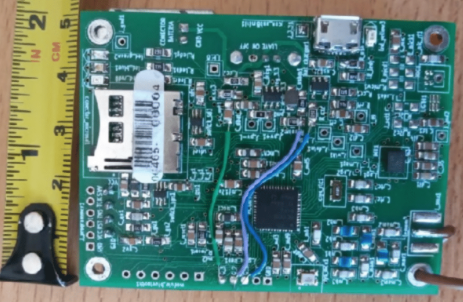
\includegraphics[width=0.75\textwidth]{dispositivo_navegacion.png}
    \caption{Dispositivo de navegación utilizado para la recolección de datos.}
    \label{fig:dispositivo_navegacion}
\end{figure}

Todos los códigos utilizados para el procesamiento de datos, entrenamiento de modelos y generación de figuras de la tesis de C. Callenbach 
están disponibles públicamente en un repositorio GitHub \cite{callenbach2025codes}.

En su trabajo logró, a partir de la utilización de herramientas de aprendizaje profundo y a partir de mediciones de campo clasificar el comportamiento 
de las tortugas en dos grupos (movimiento y quietud). Una vez se clasificaron los movimientos tiempo a tiempo, encontró que el tiempo que pasaba 
en cada uno de los estados de forma ininterrumpida seguían una distribución de ley de potencia de exponentes negativos en un rango entre $-1$ y $-2$. 
Salvo contadas excepciones para un mismo individuo, la distribución de tiempos de caminata caía de forma más abrupta que en los tiempos de espera.
Un ejemplo de estas distribuciones se muestra en la Figura \ref{fig:distribuciones}

\begin{figure}[ht]
    \centering
    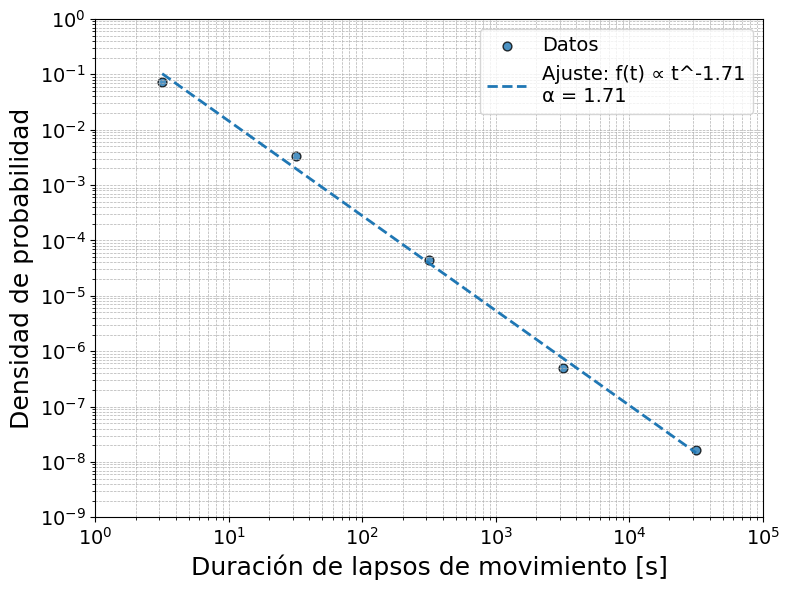
\includegraphics[width=0.45\textwidth]{distribucion_actividad_T405.png}
    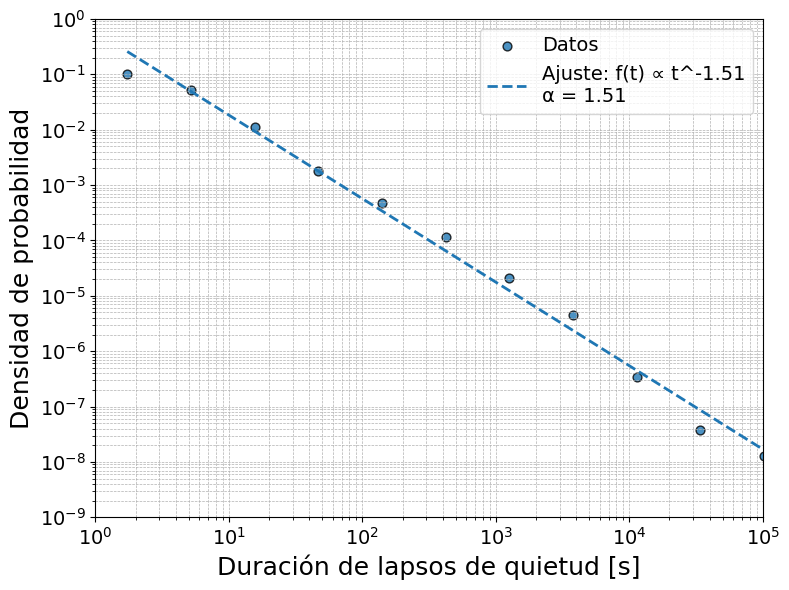
\includegraphics[width=0.45\textwidth]{distribucion_quietud_T405.png}
    \caption{Ejemplo de distribuciones de tiempos que el individuo, en este caso la tortuga T405, pasa en cada uno de los estados de forma ininterrumpida \cite{callenbach2025}.}
    \label{fig:distribuciones}
\end{figure}



\section{Datos espaciotemporales a partir de dispositivos de GPS}\label{I:GPS}

Para este trabajo se utilaron datos recolectados entre enero 2022 y febrero 2023. Durante estas campañas de campo se marca el caparazon de las tortugas para 
poder reconocerlas. Una vez se identificados los individuos se decide, teniendo en consideración la cantidad de tortugas monitoriadas y la cantidad de 
rastreadores disponibles, si se le agrega o no un dispositivo para registrar su trayectoria. Si se toma la decisión de rastrear al individuo, se le adhiere
al caparazón un dispositivo capaz de registrar las coordenadas espaciotemporales y un radiotransmisor para, al finalizar la medición, recuperar los dispositivos.
En el trabajo de tesis de M. Madille \cite{madile2023} se haya en detalle el trabajo de campaña realizado para la adquisición de datos. A continuación solo 
explicaremos el dispositivo utilizado que sirve para el trabajo desarrollado en la presente tesis.

\subsection{Unidad de navegación}

La unidad de navegación utilizada durante la campaña para la obtención de registros espaciotemporales de la ubicación de los individuos fue el dispositivo 
comercial i-gotU GT120, mostrado en la Figura \ref{fig:igotU}. Este dispositivo posee un receptor de GPS, cuya frecuencia es ajustable mediante el 
software del fabricante. La batería del dispositivo tiene una autonomía de 7 días y su peso es de $21 g$, dicho peso representa un $1.5 \%$ del peso promedio 
las tortugas, lo cual se encuentra dentro del margen deñ $5 \%$ para evitar perturbar el comportamiento. La unidad de memoria almacena posición y hora 
para cada dato adquirido, siendo accesible mediante conexión USB. 

\begin{figure}
    \centering
    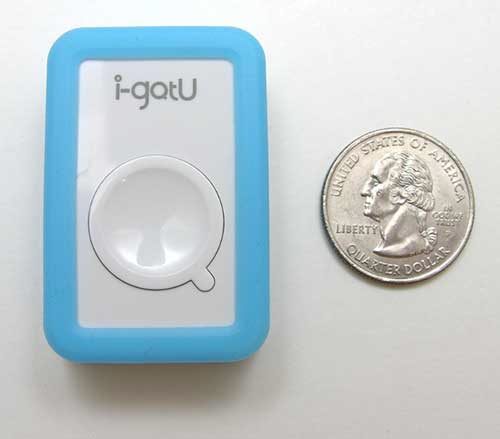
\includegraphics[width=0.45\textwidth]{IgotU.png}
    \caption{Imagen del dispositivo i-gotU, utilizado para la adquisición de datos espaciotemporales de las tortugas.}
    \label{fig:igotU}
\end{figure}

Durante esta campaña se disponía de 12 unidades de estos dispositivos, los cuales se utilizaron para medir a 6 individuos distintos, intercambiando 
los i-gotU a cada uno después de 7 días de adquisición. De esta manera se mantuvo una adquisición continua de cada una de las tortugas dado que mientras 
un dispositivo medía, su reemplazo se encontraba recargando la batería. Se programaron los dispositivos con una frecuencia de adquisición de un dato cada
15 minutos entre las 6 de la mañana y las 9 de la noche. Se evitó adquirir datos durante la noche para favorecer el ahorro de batería. Sin embargo, esta 
decisión se revirtió, tomando datos adicionales de 1am a 2am, con el objetivo de poder determinar la posición de los refugios nocturnos. La base de datos
final contó con aproximadamente 3300 horas de rastreo por tortuga.




%%% Local Variables: 
%%% mode: latex
%%% TeX-master: "template"
%%% End: 

\chapter{De los datos al modelo y del modelo a los datos}\label{Sim_diarias}
\chapterquote{}{}
\section{Introducción}\label{P:introduccion}






%%% Local Variables: 
%%% mode: latex
%%% TeX-master: "template"
%%% End: 

\chapter{Datos y mediciones a lo largo del año}\label{Datos_año}
\chapterquote{}{}



%%% Local Variables: 
%%% mode: latex
%%% TeX-master: "template"
%%% End: 

\chapter{Modelando y simulando patrones de movimiento a lo largo del año.}\label{Sim_año}
\chapterquote{}{}

\section{Introducción}\label{C:introduccion}


%%% Local Variables: 
%%% mode: latex
%%% TeX-master: "template"
%%% End: 

\chapter{Conclusiones}\label{Conclusiones}
\chapterquote{}{}


\appendix
\chapter{Apéndice 1}\label{A:1}


%%% Local Variables: 
%%% mode: latex
%%% TeX-master: "template"
%%% End: 


\begin{biblio}
\bibliography{mibib}
\end{biblio}


\begin{postliminary}

\begin{seccion}{Publicaciones asociadas}
\begin{enumerate}
  \item Presentación oral en \textbf{111va Reunión de la Asociación Física Argentina}, 2026, Catamarca, Argentina. ``Reconstruyendo el movimiento de tortugas terrestres patagónicas:  del acelerómetro al GPS''. Luciano Lopez Bertazza, Karina Laneri, Rubio-puzzo Leticia, Grigera Tomás, Kubisch Erika, Echave María Eugenia, Callenbach Tellechea Carlos
.
\end{enumerate} 
\end{seccion}
\begin{seccion}{Agradecimientos}

Grazie Mille







\end{seccion}

\end{postliminary}

\end{document}

